% Chapter 4

\chapter{Apprentissage} % 4th chapter title

\label{Chapter4} % For referencing the chapter elsewhere, use \ref{Chapter4} 

L'objectif de cette section est de reconstruire la densité de la matière en connaissant l'énergie $E$, le flux $\bvec{F}$, et la température $T$ sur les bords du domaine au cours du temps. Il s'agit donc d'un problème inverse de régression \footnote{Une classification peut tout aussi bien être implémentée (voir paragraphe \ref{sec:Classif}). Sauf mention du contraire, lorsqu'on parlera d'apprentissage, il s'agira du problème de régression.}, la densité faisant partie des paramètres du problème direct; et les signaux temporels $E$, $\bvec F$, et $T$ faisant partie des résultats. Nous ferons une simplification de taille : \textbf{la densité est un signal en créneau lissé} \footnote{Un créneau sur la densité sera aussi appelé saut de densité, ou pic de densité, ou obstacle sur la densité} (on utilisera un créneau cylindrique i.e ayant la forme d'un cercle de diamètre 0.1 vu du haut). Ainsi, reconstruire la densité revient juste à prédire la position et la hauteur du créneau. La valeur de la densité en dehors du créneau sera connue. 

Nous recherchons donc une fonction $f^{-1}$ (inverse de la fonction $f$ définissant le problème direct) telle que $y = f^{-1}(\bvec{X})$. Où $y$ représente la densité de la matière (plus précisément les attributs de son créneau), et $\bvec{X}$ les signaux sur les bords. Le caractère généralement mal posé des problèmes inverses rend difficile la détermination de $f^{-1}$. On procède donc à une approximation de $f^{-1}$ notée $\hat{f}^{-1}$, par apprentissage supervisé\footnote{Un apprentissage automatique pour lequel les exemples (ou « samples ») sont annotés par des labels.} à l'aide d'un ANN \footnote{Réseau de neurones artificiel}. En notant $\bm{\theta}$ les paramètres de l'ANN, on cherche $\hat{y}$ telle que $ \hat{y} = \hat{f}^{-1}(\bvec{X}, \bm{\theta}). $

%----------------------------------------------------------------------------------------

\section{Description des entrées/sorties}

Il s'agit dans cette partie de décrire les entrées et les sorties qui ont été obtenues durant l'étape (préliminaire à apprentissage) de génération des données. En 1D le domaine est $[0,1]$ discrétisé sur 300 mailles, et en 2D le domaine est $[0,1] \times [0,1]$ discrétisé sur 28x28 mailles. Cependant les données 1D et 2D se partagent un certain nombre de paramètres, principalement composé des paramètres physiques du problème :
\begin{itemize}
  \item temps final = 0.01 \si{sh} \textit{(1 shake (\si{sh}) = $10^{-8}$ secondes)}
  \item $c = 299$ [\si{\cm \per sh}]
  \item $a = 0.01372$ [\si{g \per cm \per sh^2  \per keV }]
  \item $C_v = 0.14361$ [\si{Jerk \per\g \per keV}] \textit{(1 \si{Jerk} = 1\si{m \per \s\cubed})}
  \item la densité $\rho$ est un signal en créneau [\si{\g\per\cm\cubed}]
  \item $\sigma_a = \rho T$ [\si{\per\cm}]
  \item $\sigma_c = \rho T$ [\si{\per\cm}]
  \item $T_0 = 5$ [\si{keV}] \textit{(en termes de température, 1 \si{keV} = 11605 \si{K})}
  \item $E_0 = 0.01372\times 5^4$ [\si{g \per \cm \per sh^2}]
  \item $\bvec{F}_0 = \bvec{0}$ [\si{g \per sh^2}]
\end{itemize}

La situation initiale pour chacune des simulations effectuées correspond à l'équilibre radiatif ($E_0=aT_0^4$, i.e température initiale de la matière ($T_0$) = température initiale de la radiation ($Tr_0$) = $(E_0/a)^{1/4}$). La situation sur une portion de la gauche correspond à cet équilibre perturbé par une source sinusoïdale ($ E_{gauche} = aT_{0}^4 + 5 \sin (2 k \pi t) $)\footnote{Toute la gauche est naturellement couverte par la source en 1D, avec $k=1000$. En 2D, $k=500$} (condition de Dirichlet). Sur le reste de la gauche (en 2D), l'équilibre radiatif est maintenu (condition de Dirichlet). Les situations sur les autres bords (1 en 1D et 3 en 2D) correspondent à des sorties libres (condition de Neumann).

À quelques différences près (nombre de mailles, position de la source sur la gauche), la figure \ref{fig:SimuCFG} représente un exemple typique de configuration utilisé en 2D (les paramètres physiques applicables en 1D peuvent aussi être observés). La définition des fichiers de configurations pour la 1D et la 2D est définie sur leur dépôt Github respectifs (voir annexe \ref{AppendixA}).


\subsection{En 1D}
L'aspect d'une entrée et d'une sortie 1D est représentée à la figure \ref{fig:entreesortie1D}. Les entrées sont composées des signaux temporels $E$, $\bvec{F}$, et $T$. Suivant chacun de ces canaux, il faut normaliser les entrées avant de les nourrir au réseau de neurones. Vu que le signal provient de la gauche, les entrées ne sont constituées que du signal récupéré sur le bord droit du domaine. La talle d'un exemple est présentée à la figure \ref{fig:entrees1D}. 

\begin{figure}[!h]
\centering
\includegraphics[width=.6\linewidth]{entreesortie1D} 
\decoRule
\caption[entreesortie1D]{Visualisation d'une entrée de l'ANN (en haut) et d'une sortie (en bas) en 1D. Seul le signal sur la droite du domaine est utilisé. Tout les 3 canaux $E$, $\bvec{F}$ et $T$ sont représentés ici.}
\label{fig:entreesortie1D}
\end{figure}

\begin{figure}[H]
\centering
\includegraphics[width=.4\linewidth]{entrees1D} 
\decoRule
\caption[entrees1D]{Taille d'une entrée 1D. La dimension temporelle (nombre d'itérations) a été ré-échantillonnée de 907 à 50. Les 3 canaux désignent les signaux $E$, $\bvec{F}$ et $T$.}
\label{fig:entrees1D}
\end{figure}

Comme mentionné plus haut, nous avons fait quelques simplifications sur la nature de la sortie. Il s'agit d'un vecteur de seulement deux scalaires\footnote{Les deux scalaires sont extraits de l'image du bas de la figure \ref{fig:entreesortie1D}} représentant la position et la hauteur du saut de densité :
\begin{itemize}
 \item \textbf{Position} : il s'agit de l'abscisse de l'obstacle choisi de façon à ce que le créneau se situe entièrement dans le domaine (i.e position de son centre comprise dans l'intervalle $[0.07,0.92]$).
 \item \textbf{Hauteur} : comprise dans l'intervalle $[1.05, 9.99]$. La valeur de la densité en dehors du créneau est de 1.
\end{itemize}


\subsection{En 2D}
Une entrée 2D contient considérablement plus d'information qu'une entrée 1D. Les 3 signaux $E$, $\bvec{F}$ et $T$ sur les 4 bords sont inclus. On y ajoute chacun des groupes de signaux correspondants aux 4 positions de la source sur la gauche. En effet, une entrée correspond à 4 simulations effectuées chacune avec la source à une position différente, comme on peut le voire à la figure \ref{fig:entreesortie2D}. La taille d'une entrée est donnée à la figure \ref{fig:entrees2D}.

\begin{figure}[!h]
\centering
\includegraphics[width=.95\linewidth]{entreesortie2D} 
\decoRule
\caption[entreesortie2D]{Visualisation d'une entrée (aux alentours de chacune des quatre images) et d'une sortie (aux milieux) en 2D. On peut voire les postions des 4 sources (sur la gauche) utilisées à tour de rôle pour former une seule entrée. Ici n'est représentée que l'énergie (qui constitue 1/3 des canaux) sur les 4 bords. Les images des densités ci-contre ont été obtenues par interpolation bilinéaire d'une image initiale très grossière (28x28).}
\label{fig:entreesortie2D}
\end{figure}

\begin{figure}[!h]
  \centering
  \includegraphics[width=.5\linewidth]{entrees2D} 
  \decoRule
  \caption[entrees2D]{Taille d'une entrée en 2D. Contrairement à la 1D, il faut tenir compte de la dimension spatiale qui correspond au nombre de mailles sur chaque bord du domaine rectangulaire ($N=M=28$). Le nombre de canaux passe à 48 car il faut dejà tenir compte des 3 canaux originaux ($E$, $\bvec{F}$, et $T$), ensuite de chacun de 4 bords du domaine, et enfin des 4 positions de la source.}
  \label{fig:entrees2D}
\end{figure}

Compare à la 1D, il faut rajouter l'ordonnée du saut de densité à la liste des scalaires prédits. Une sortie donc est un vecteur de taille 3. Afin d'éviter des cas trop extrêmes, les valeurs observées (ou labels pour l'apprentissage) sont convenablement choisies au moment de la génération des données :
\begin{itemize}
 \item \textbf{Abscisse} : comprise dans l'intervalle $[0.2,0.8]$ afin de récupérer une réponse non aberrante sur chacun des 4 bords du domaine.
 \item \textbf{Ordonnée} : comprise aussi dans l'intervalle $[0.2,0.8]$.
 \item \textbf{Hauteur} : comprise dans l'intervalle $[0.1,10]$. La valeur 0.1 est aussi la valeur de la densité en dehors de son créneau. Cette valeur faible permet d'éviter l'absorption complète de l'onde sur le domaine.
\end{itemize}

En 1D comme en 2D, il faudra séparer le jeu de données en 3 parties avant de procéder à l'apprentissage :
\begin{itemize}
  \item \textbf{train}: il s'agit des données utilisées pour l'entrainement du modèle d'ANN construit.
  \item \textbf{val}: pour évaluer la qualité d'une époque de l'entrainement.
  \item \textbf{test}: pour tester le modèle. Les scores que nous présenterons seront calculés sur ces données. 
\end{itemize}

Des jeux de données complets 1D/2D ont été sauvegardés sur Github; et les détails pour les récupérer et les traiter sont donnés en annexe \ref{AppendixB}.

%----------------------------------------------------------------------------------------

\section{Architecture générale}

Un réseau de neurones artificiel \footnote{Ou juste réseau de neurones dorénavant} (ANN) est un système computationnel basé sur le réseau de neurones biologique. L'apprentissage profond, à travers ses réseaux de neurones profonds\footnote{Réseaux de neurones composé d'un nombre relativement élevé de couches cachées} (DNN\footnote{Deep Neural Network}), permet de résoudre des problèmes en Machine Learning que les méthodes classiques (régression linéaire, SVM, etc.) ne peuvent pas. Il réussit cela en introduisant des représentations des données qui s'expriment sous forme d'autres représentations, plus simples cette fois. 

Les réseaux profonds en aval\footnote{En opposition à un réseau de neurones récurrent qui réutilisent les résultats de son modèle pour s'améliorer.} (ou MLP \footnote{Multi-Layer Perceptron}) constituent l'exemple de choix en apprentissage profond. On peut l'interpréter comme une fonction (plus exactement une composition de fonctions : $f^{-1} = f_1 \circ f_2 \circ \cdots \circ f_n$) faisant correspondre une série d'entrées à une sérié de sorties. Il est constitué de plusieurs couches (assimilables aux fonctions $f_1$, $f_2$, .., $f_n$ précédentes) apprenant chacune un aspect particulier des données. On distingue une couche d'entrée, une ou plusieurs couches cachées, et une couche de sortie (voir figure \ref{fig:MLP}).


\begin{figure}[!h]
\centering
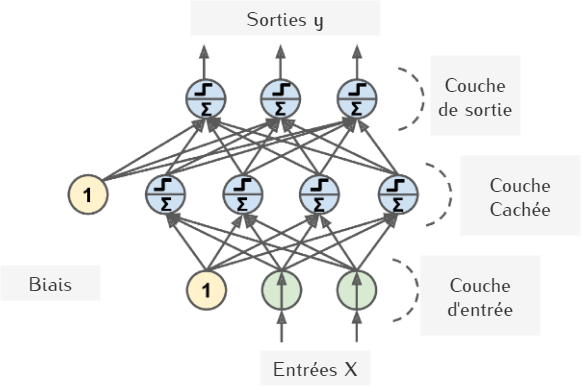
\includegraphics[width=.6\linewidth]{MLP} 
\decoRule
\caption[MLP]{Illustration d'un MLP avec une couche cachée. Le nombre de couches cachées peut être élevée ce qui conduit aux DNN. Le 1 représente le biais \parencite[286]{Reference8}.}
\label{fig:MLP}
\end{figure}

Les réseaux de neurones convolutifs (CNN) sont une forme de MLP spécialisés dans le traitement des données en forme de grille. Par exemple des séries en temps qui peuvent êtres vues comme des grilles 1D (l'axe de temps) prenant des données (vecteur de données) à intervalle de temps régulier \parencite{Reference5}. Ils sont donc particulièrement adaptés à la reconstruction de la densité partant des signaux temporels $E$, $\bvec{F}$, et $T$. 

L'architecture de CNN de base pour notre apprentissage a été proposée par M. \textsc{Vigon}. Nous utiliserons deux variantes : DRNN \footnote{Density Reconstruction Neural Network} 1 (figure \ref{fig:DRNN1}) et DRNN 2 (figure \ref{fig:DRNN2}). Les architectures seront implémentées sous la librairie de Machine Learning Keras (avec le « backend » TensorFlow). Les différentes couches présentées seront détaillés dans la suite. Nous indiquerons aussi en quoi elles sont importantes pour notre apprentissage.

\begin{figure}[!h]
\centering
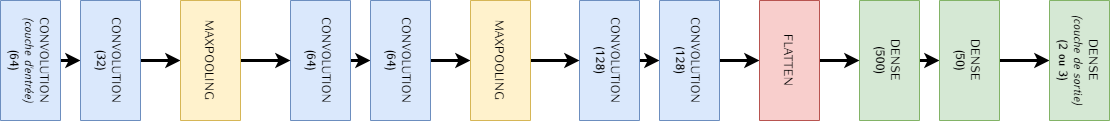
\includegraphics[width=.95\linewidth]{DRNN1}
\decoRule
\caption[DRNN1]{Première architecture (nommée DRNN 1). Le nombre de neurones utilisés pour chaque couche est indiqué entre parenthèses. Le nombre de neurones de la couche de sortie dépend qu'on soit en 1D ou en 2D.}
\label{fig:DRNN1}
\end{figure}

\begin{figure}[H] 
\centering
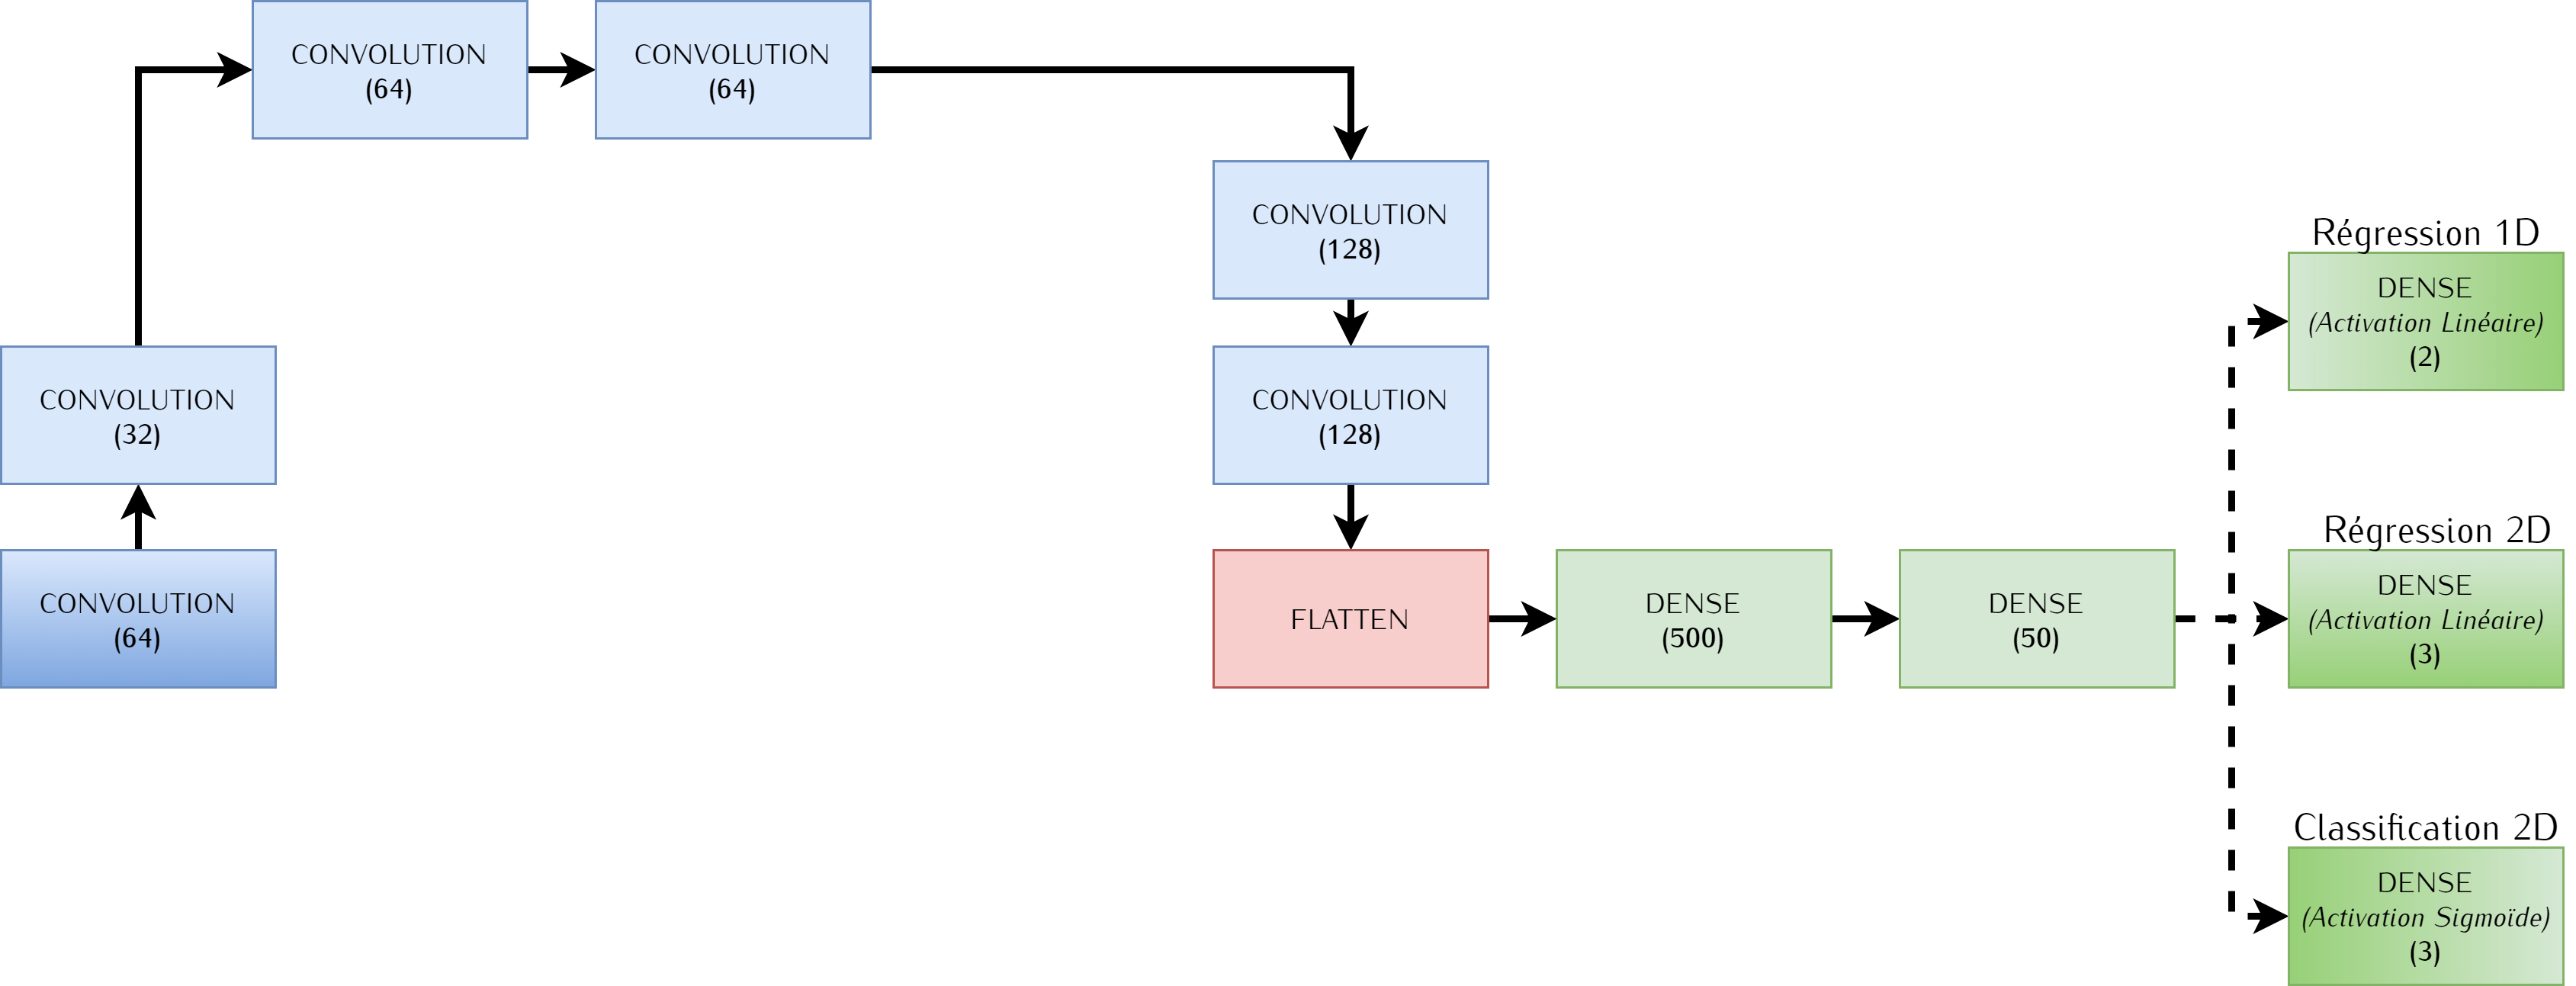
\includegraphics[width=.95\linewidth]{DRNN2} 
\decoRule
\caption[DRNN2]{Deuxième architecture utilisée (nommée DRNN 2). Ce modèle ne contient pas de couche de « pooling » \footnotemark.}
\label{fig:DRNN2}
\end{figure}
\footnotetext[6]{Les détails concernant l'opération de « pooling » seront donnés à la section \ref{subsec:MaxPoling}}

% \clearpage
% \begin{figure}[h!]
%    \begin{minipage}{0.6\textwidth}
%      \centering
%      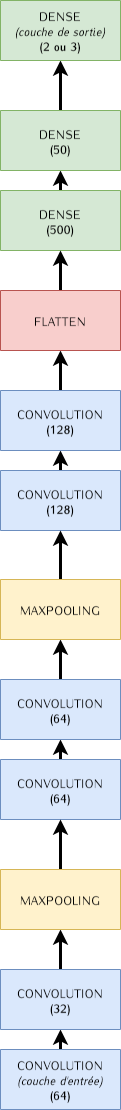
\includegraphics[width=.2\linewidth]{DRNN1ROT}
%      \decoRule
%      \caption[DRNN1]{Première architecture (nommée DRNN 1). Le nombre de neurones utilisés pour     
%      chaque couche est indiqué entre parenthèses. Le nombre de neurones de la couche de sortie 
%      dépend qu'on soit en 1D ou en 2D.}
%      \label{fig:DRNN1}
%    \end{minipage}\hfill
%    \begin{minipage}{0.4\textwidth}
%      \centering
%      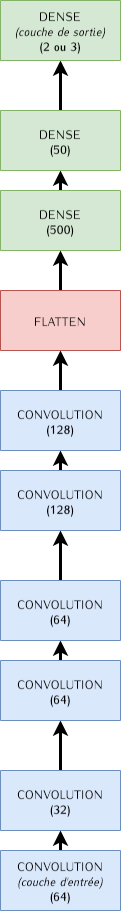
\includegraphics[width=.3\linewidth]{DRNN2ROT}
%      \decoRule
%      \caption[DRNN2]{Deuxième architecture utilisée (nommée DRNN 2). Ce modèle ne contient pas de 
%      couche de « pooling » \footnotemark }
%      \label{fig:DRNN2}
%    \end{minipage}
% \end{figure}
% \footnotetext[6]{Les détails concernant l'opération de « pooling » seront donnés à la section \ref{subsec:MaxPoling}}

% \begin{figure}[!ht]
% \begin{subfigure}{.6\textwidth}
%   \centering
%   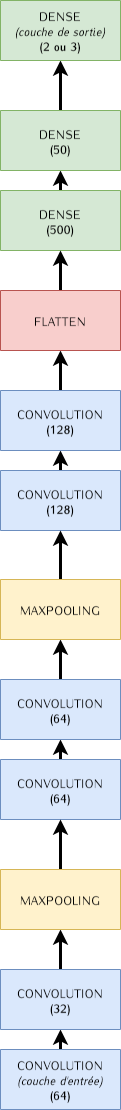
\includegraphics[width=.2\linewidth]{DRNN1ROT}  
%   \caption[DRNN1]{CPremeire architecture (nommee DRNN 1 ). Le nombre de neurones utilisés pour     
%      chaque couches est indiques entre parentheses. Le nombre de neurnoes de la couche de sortie 
%      depend qu'on soit en 1D ou en 2D.}
%   \label{Fig:DRNN1}
% \end{subfigure}
% \begin{subfigure}{.4\textwidth}
%   \centering
%   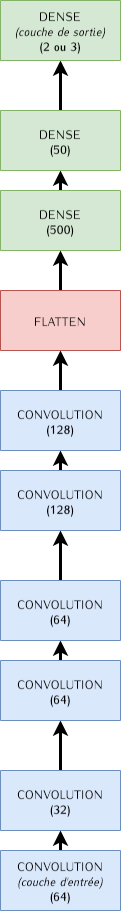
\includegraphics[width=.3\linewidth]{DRNN2ROT}  
%   \caption[Conv2D]{Deuxieme architecture utilisee (nommee DRNN 2). Ce modlee ne contient pas de 
%      couches de Pooling \footnote{Les details concernant le pooling seront données a la section \ref{subsec:MaxPoling}}}
%   \label{Fig:DRNN2}
% \end{subfigure}
% \label{Fig:DRNN}
% 
% \centering
% \decoRule
% \caption[DRNN]{Differents modeles de CNN utilisés}
% \end{figure}
% 

% ----------------------------------------------------------------------------------------
% \newpage
\section{Les couches utilisées}

\subsection{Les couches de convolution}
La convolution est l'opération fondamentale d'un CNN. Il s'agit d'une opération linéaire qui combine deux signaux pour en extraire un troisième. En général, une opération de convolution se définit par la formule suivante ($i$ est le signal d'entrée et $k$ est le noyau de la convolution) :
$$ s(t) = (i * k)(t) = \int i(x)k(t-x) \, dx $$

En pratique, les signaux temporels ne sont pas continus, ils sont discrétisés par intervalles de temps $\Delta t$. Dans ce contexte, la convolution 1D se définit par la formule :
\begin{equation}
 s(t) = \sum_{x=-\infty}^{\infty} i(x)k(t-x)
 \label{eqn:Conv1D}
\end{equation}

Cette formule doit être adaptée en 2D vu qu'on fera aussi un apprentissage 2D. La formule devient donc :
\begin{equation}
 S(i,j) = (I * K)(i,j) = \sum_{m}\sum_{n} I(m,n)K(i-m,j-n)
 \label{eqn:Conv2D}
\end{equation}

L'opération de convolution est commutative grâce à l'inversion du noyaux relativement par rapport au signal d'entrée. Cette propriété, bien qu'importante d'un point de vue théorique, ne présente pas d'avantages du point de vue computationnel. C'est la raison pour laquelle on dispose de l'opération de cross-corrélation qui est une convolution sans inversion du noyau. En 2D elle se présente comme ceci :
\begin{equation}
 S(i,j) = (I * K)(i,j) = \sum_{m}\sum_{n} I(i+m,j+n)K(m,n)
 \label{eqn:Corr2D}
\end{equation}

On remarque aussi que le parcours des indices se fait suivant l'input. Il se trouve que c'est plus direct et rapide ainsi, parce qu'il y a moins de variation dans la plage de valeurs valides pour $m$ et $n$ \parencite[322ff.]{Reference5}. 

Plusieurs librairies de Machine Leanring implémentent la cross-corrélation mais l'appellent convolution. C'est le cas de Keras lorsqu'elle utilise le « backend » TensorFlow \footnote{Lorsqu'on utilise Theano, les convolutions sont effectivement des convolution comme definie en \ref{eqn:Conv1D} et \ref{eqn:Conv2D}.} \parencite{Reference6}.
% 
% \begin{figure}[!h]
%     \subfloat[Convolution 1D]{
%    \begin{minipage}{0.5\textwidth}
%      \centering
%      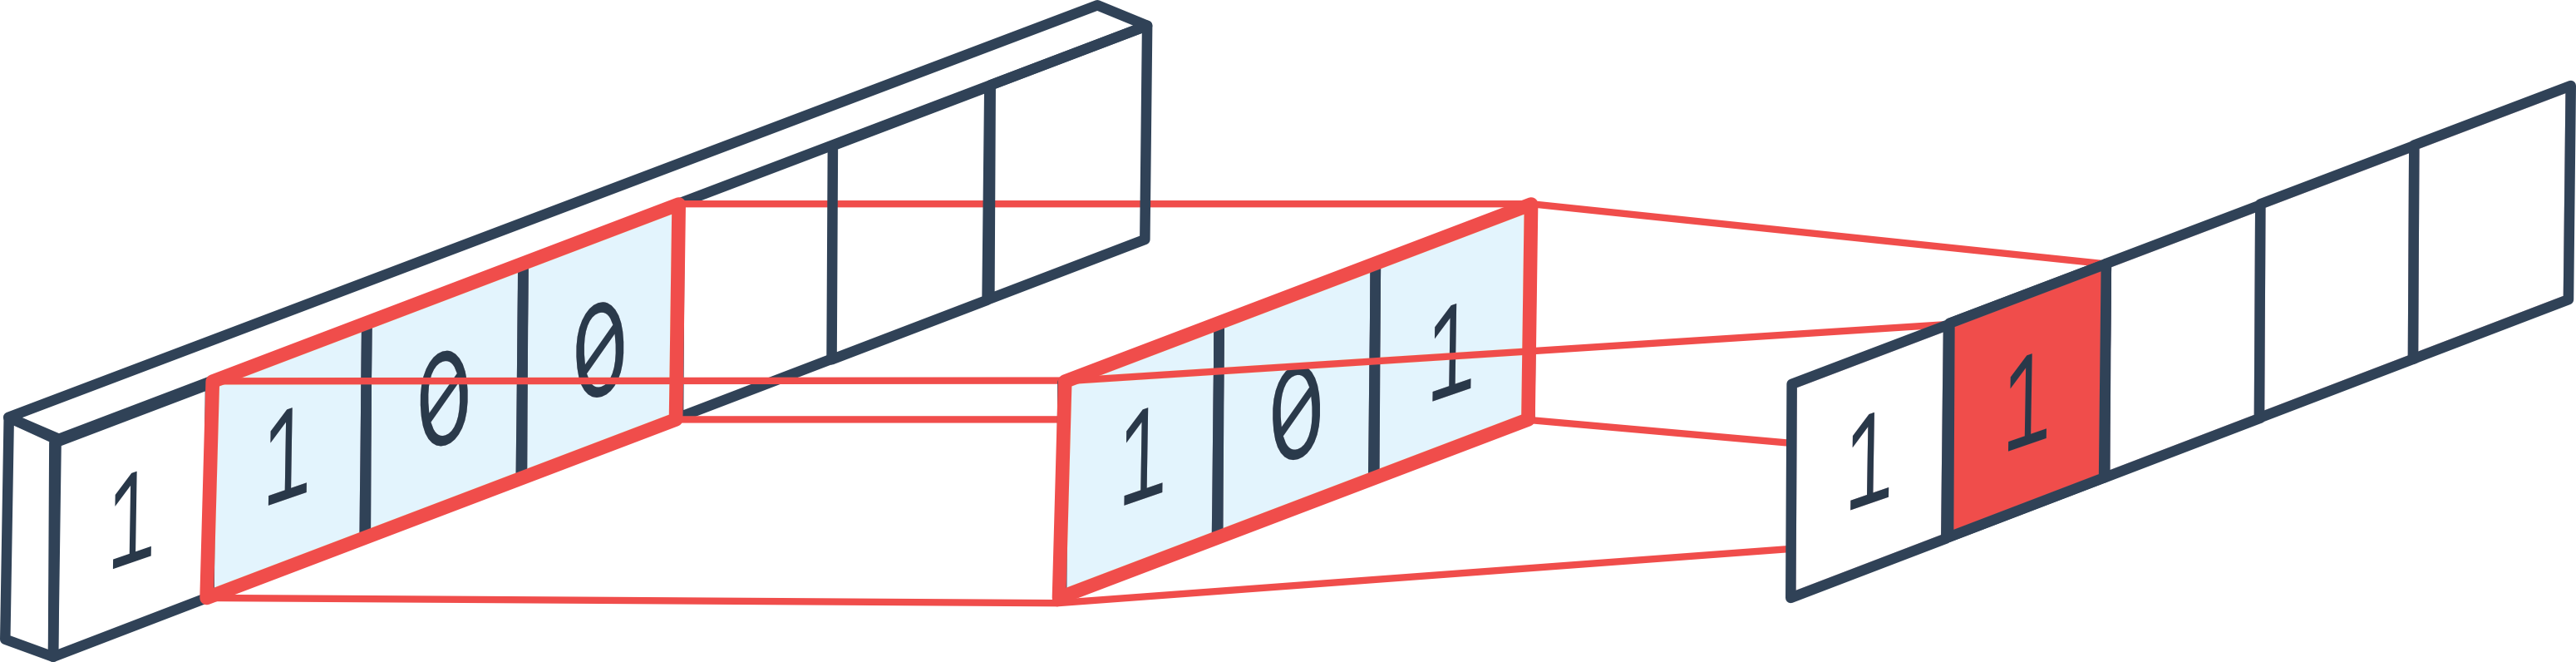
\includegraphics[width=.95\linewidth]{Conv1D}
%    \end{minipage}}
%    \hfill
%    \subfloat[Convolution 2D]{
%    \begin{minipage}{0.5\textwidth}
%      \centering
%      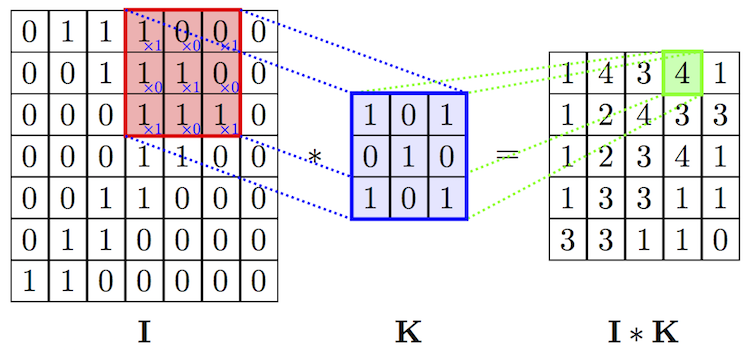
\includegraphics[width=.95\linewidth]{Conv2D}
%    \end{minipage}}
%    \label{Fig:Conv1D2D}
% 
%    \centering
%    \decoRule
%    \caption[Conv2D]{Illustration d'une convolution (cros-corelation) 1D/2D en mode "valide" (aucun padding de 0 ne sera ajoute et la sortie S aura une taille inferieure a l'entree I). La taille du noyaux que nous utiliserons sera de 3 (1D) et (6,2) (2D) . Un autre paramtre important pour reduire la taille de la sortie est le "stride", il s'agit de l'ecart entre deux applications du noyaux de convolution K. Nous le prenons egale a 1 (1D) et (1,1) (2D) de facon a couvrir tous les indices valides de l'entree I.}
% \end{figure}


\begin{figure}[!h]
\begin{subfigure}{.5\textwidth}
  \centering
  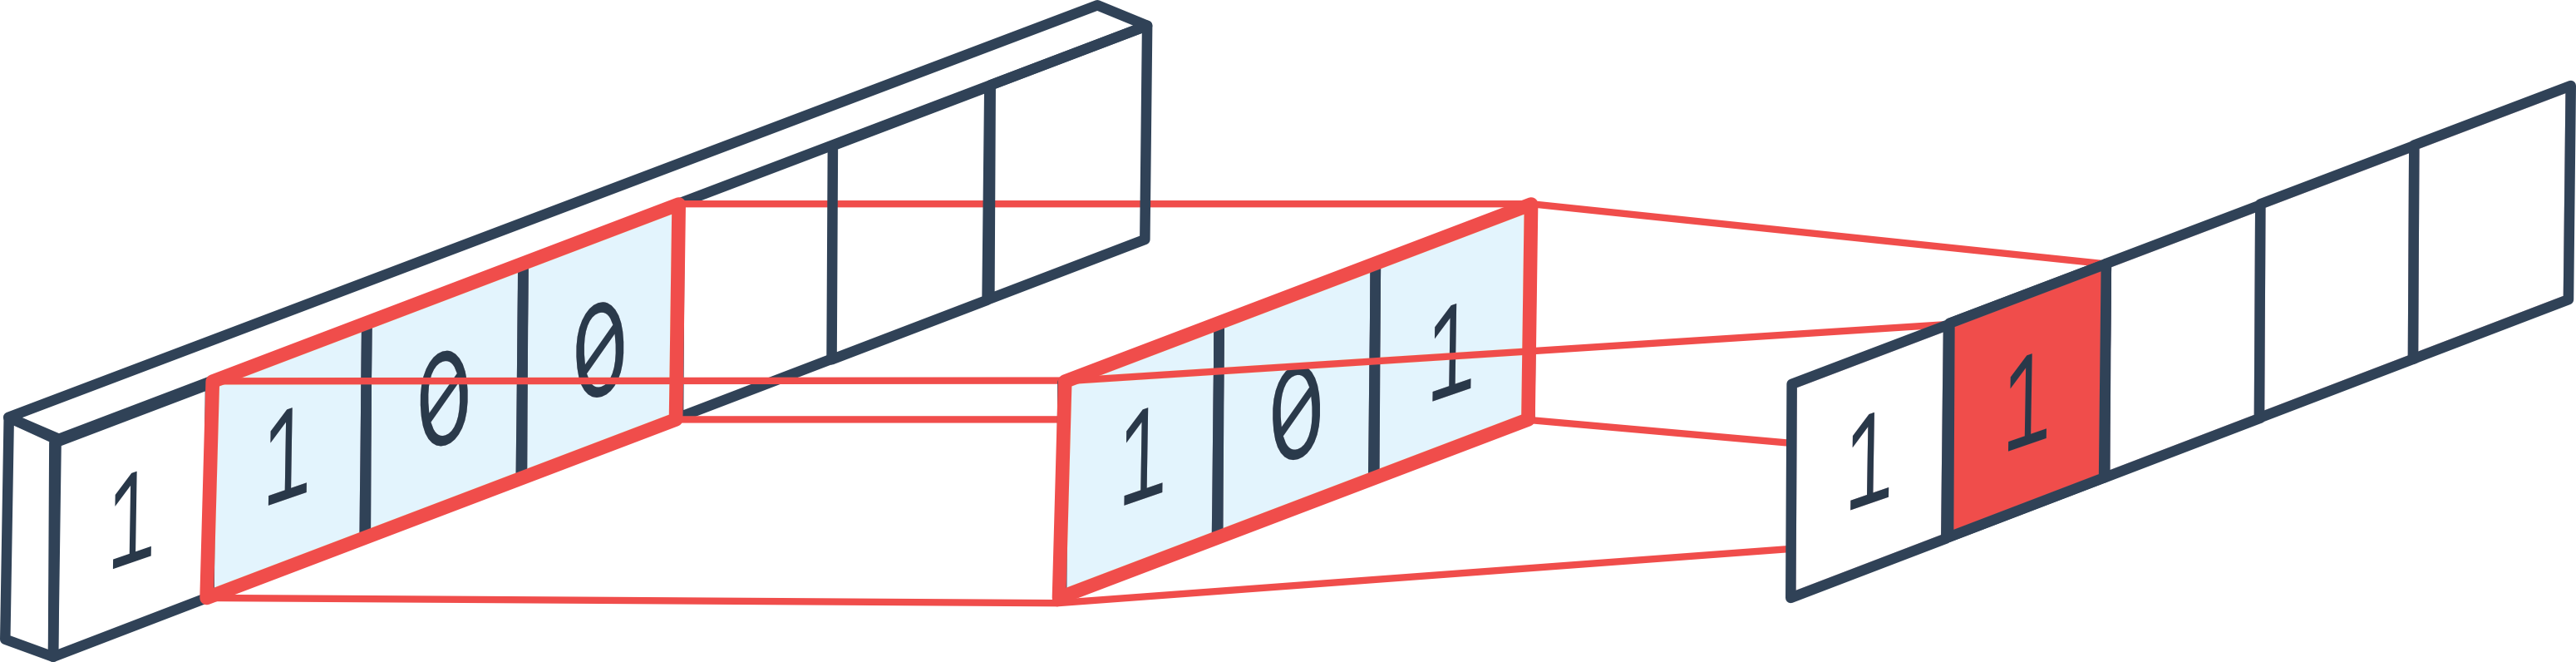
\includegraphics[width=.95\linewidth]{Conv1D}  
  \caption[Conv1D]{Convolution 1D \parencite{Reference10}}
\end{subfigure}
\begin{subfigure}{.5\textwidth}
  \centering
  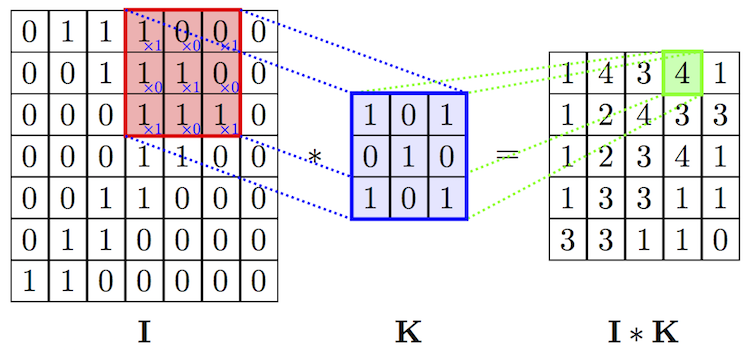
\includegraphics[width=.95\linewidth]{Conv2D}  
  \caption[Conv2D]{Convolution 2D \parencite{Reference11}}
\end{subfigure}
\label{fig:Conv1D2D}

\centering
\decoRule
\caption[Convolution1D2D]{Illustration d'une convolution (cross-corrélation) 1D/2D en mode "valid" (aucun « padding » de 0 ne sera ajouté et la sortie $S$ aura une taille inférieure à l'entrée $I$). La taille du noyaux que nous utiliserons sera de 3 (en 1D) et (6,2) (en 2D). Un autre paramètre important pour réduire la taille de la sortie est le "stride"; il caractérise de l'écart entre deux applications consécutives du noyaux de convolution $K$. Nous le prenons égale à 1 (en 1D) et (1,1) (en 2D) de façon à couvrir tous les indices valides de l'entrée $I$.}
\end{figure}

% 
% Les CNN apportent trois notions cles a un apprentissage:
% \begin{itemize}
%  \item l'interaction creuse: contrairemetn aux couches traditionneles, les couches de convolution utilisent des noyaux de taille condiereblemen inferieure a celle de l'input. En terme de multiplication matricielle, cela permet de faire des taches toutes aussi importantes (detection des condouts, floutage, etc..) en ne gardant que peu de parametres en memoire et augmentant l'efficacite statitique. Cela permet aussi de reduire les couts de calcul.
%  (IMAGE)
%  \item le partage des parametres: les coefficient du noyau de convolution sont reutilisés a chaque endroit de la matrice d'entree, contrairement aux couches traditionnelles qui utilise generalement chaque coefficient une seule fois.
%  (IMAGE)
%  \item la representation equivariante: le partage de parametre introduit la proprite d'equivaraition par translation. SI l'entree change, la sortie change de la meme facon, et le reseau de neurones exploite cela. Par exemple, dans l'etude d'une image, il serait interressant de detecter les contour dans la premiere couche du reseau,vu que ces meme contour sont suceptibles de reaparatire dans la suite. (\parencite{Reference5})
% \end{itemize}


Dans les architecture de CNN typiques, l'opération de convolution est généralement suivi d'une étape dite de détection. Dans cette étape, les résultats de la convolution (linéaires) sont passés à une fonction non linéaire au niveau d'une couche d'activation. Nous détaillerons la notion d'activation dans les sections suivantes. Après cette étape de détection, le Pooling est généralement appliqué pour modifier les résultats encore plus profondément.

\subsection{Le Max-pooling}
\label{subsec:MaxPoling}
L'opération de Pooling permet de réduite la taille des données (« downsampling »). Une fonction de Pooling transforme les entrées voisines par une fonction d'agrégation statistique. Plusieurs fonctions d'agrégations peuvent êtres utilisées. Par exemple, le Max-pooling renvoi le maximum sur un domaine appelé « pool size » (rectiligne en 1D et rectangulaire en 2D). 


\begin{figure}[!h]
\begin{subfigure}{.5\textwidth}
  \centering
  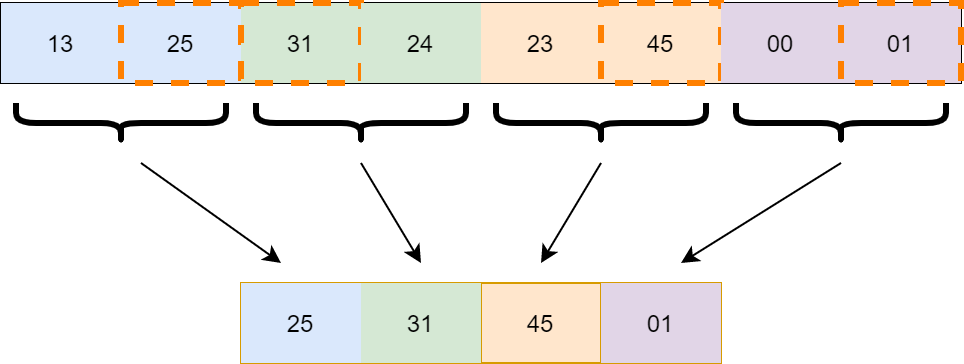
\includegraphics[width=.95\linewidth]{MaxPool1D}  
  \caption[MaxPool1D]{Max-pooling 1D}
\end{subfigure}
\begin{subfigure}{.5\textwidth}
  \centering
  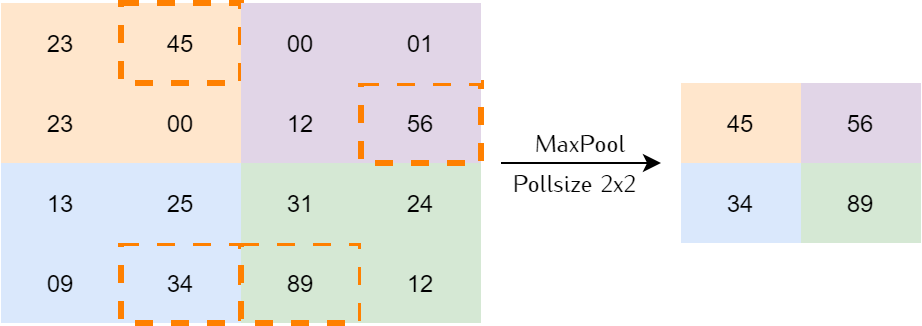
\includegraphics[width=.95\linewidth]{MaxPool2D}  
  \caption[MaxPool2D]{Max-pooling 2D}
\end{subfigure}
\label{fig:MaxPool1D2D}

\centering
\decoRule
\caption[MaxPoling]{Opération de Max-pooling en 1D/2D avec un « pool size » de 2 (en 1D) et de 2x2 (en 2D).}
\end{figure}


En général, l'opération de Pooling permet de rendre la représentation approximativement invariante aux petites variations dans l'input. Parlant de l'identification d'objets dans une image par exemple, « L'invariance par translations locales (petites translations) peut être utile si on est plus intéressé par la présence de l'objet que par sa localisation exacte. »\parencite[330]{Reference5}.

Dans le problème inverse que nous résolvons, on aimerait non seulement détecter la présence du saut de densité, mais aussi ses coordonnées exactes. Cela nous amène donc à considérer dans un premier temps une architecture avec Max-pooling (figure \ref{fig:DRNN1}), et dans un deuxième temps, sans Max-pooling (figure \ref{fig:DRNN2}).
 
\subsection{Flatten}
L'opération d'aplatissage (ou Flatten) permet de transformer les données en quittant de la forme tensorielle (2D avec plusieurs canaux) à une forme vectorielle. Il s'agit en réalité d'une étape de préparation pour les couches denses (complètement connectées).

\begin{figure}[!h] 
\centering
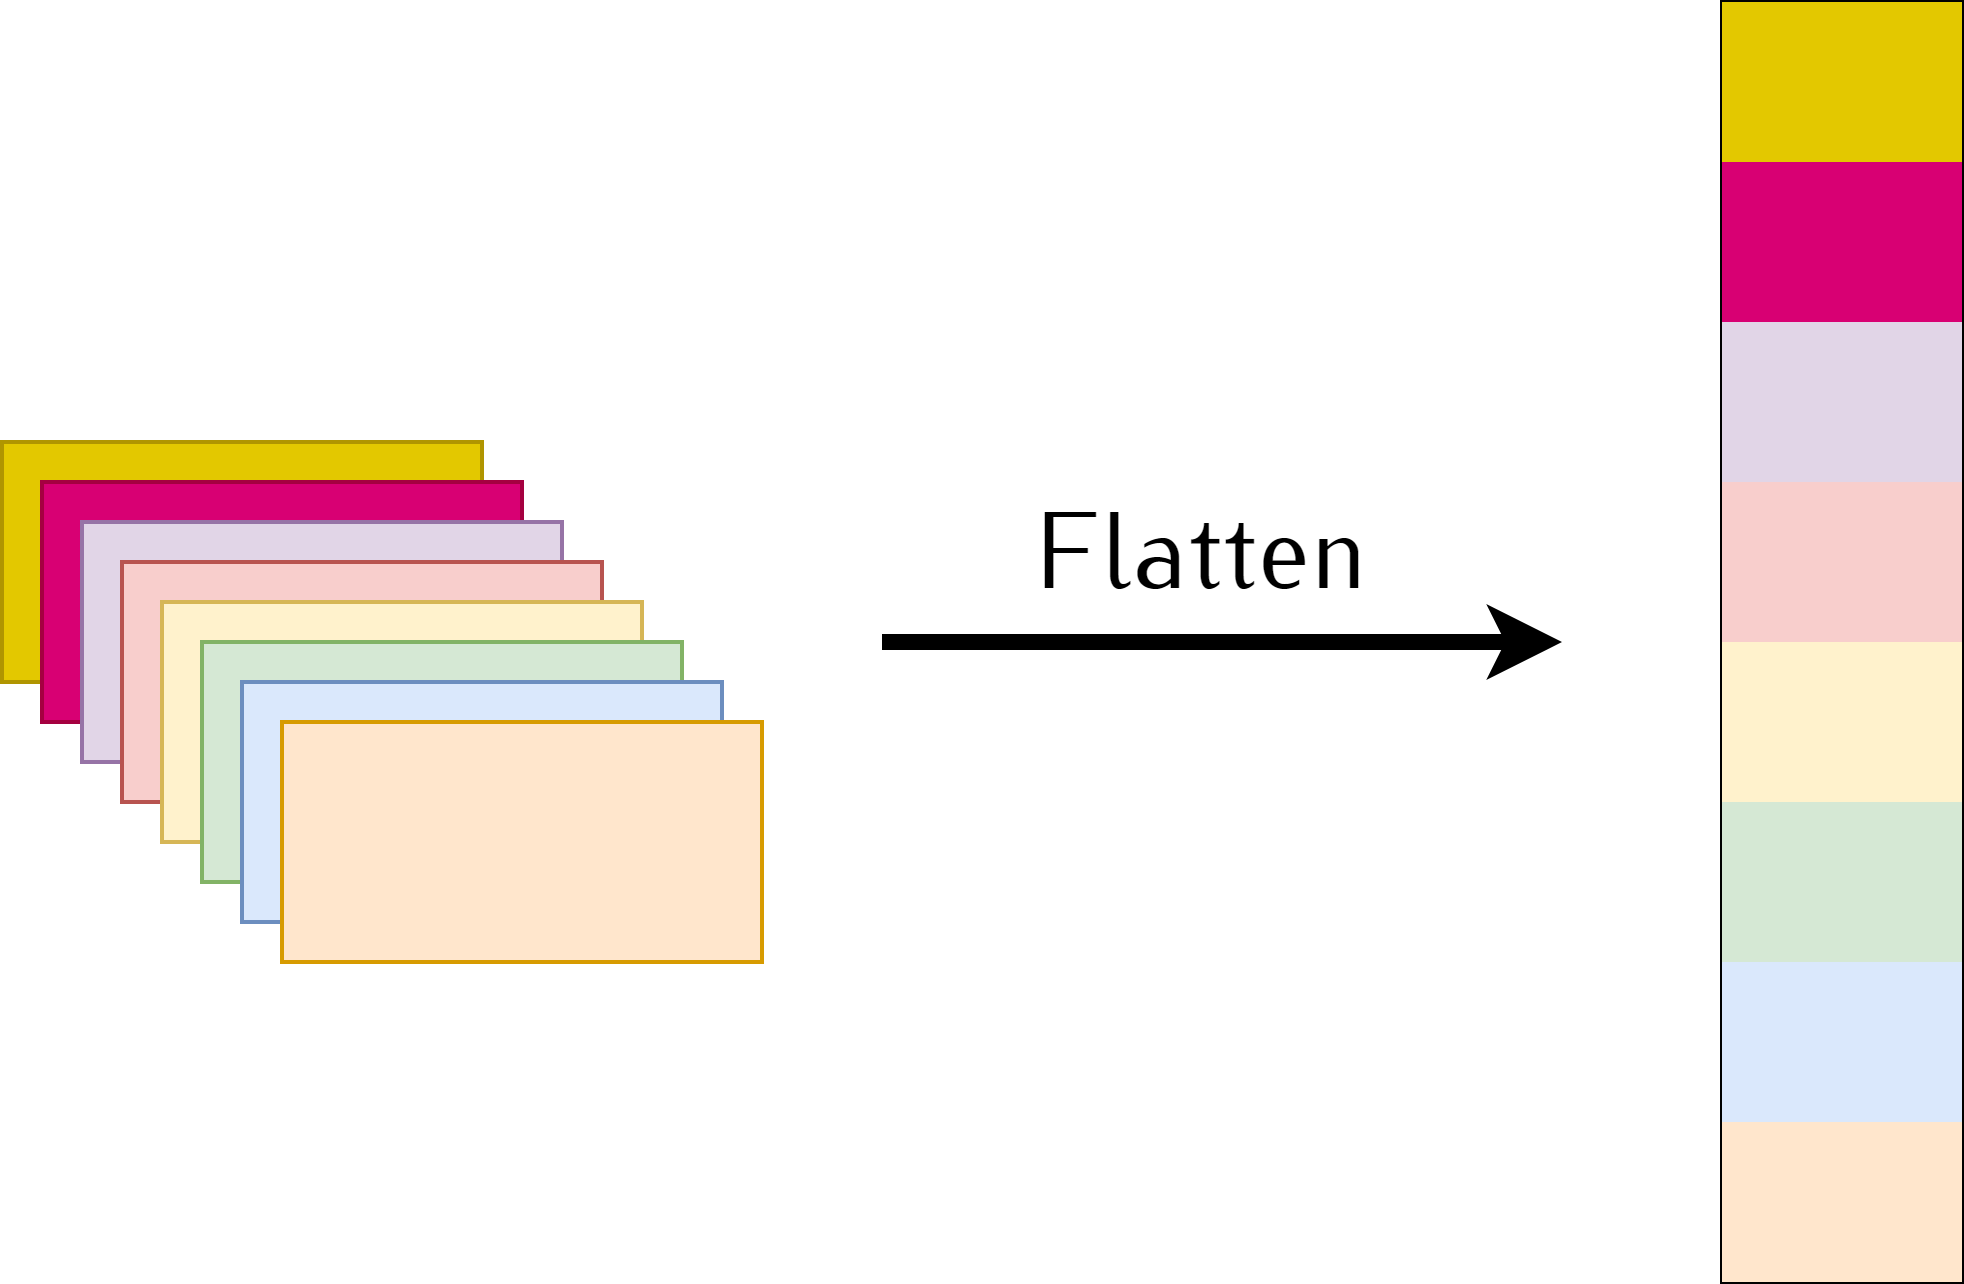
\includegraphics[width=.5\linewidth]{Flatten}
\decoRule
\caption[Flatten]{Illustration d'une opération de Flatten). Qu'on soit en 1D ou en 2D, le Flatten assure que sa sortie est un vecteur sur lequel une couche dense peut opérer.}
\label{fig:Flatten}
\end{figure} 

\subsection{Les couches denses}
À ce niveau, tous les neurones d'une couche sont connectés à tous les neurones de la couche précédente. Une couche dense (ou « fully connected ») prend les résultats d'une convolution/Pooling et en ressort des poids. Les couches de convolution ayant appris des aspects particuliers des données, la couche dense est un moyen relativement facile d'apprendre des combinaisons de ces dernières.

Si $f_i$ désigne la fonction représentant une couche dense, l'opération effectuée est $f_i(\bvec X)=\phi(\bvec X \mathsf{W} + \bvec b)$, où $\bvec X$ représente les entrées de la couche, $\bvec b$ le biais, $\mathsf{W}$ la matrice des poids (une ligne par neurone d'entrée et une colonne par neurone de cette couche, excepté ceux du biais), et $\phi$ la fonction d'activation que nous détaillerons plus tard. \parencite[286]{Reference8}

\begin{figure}[!h] 
\centering
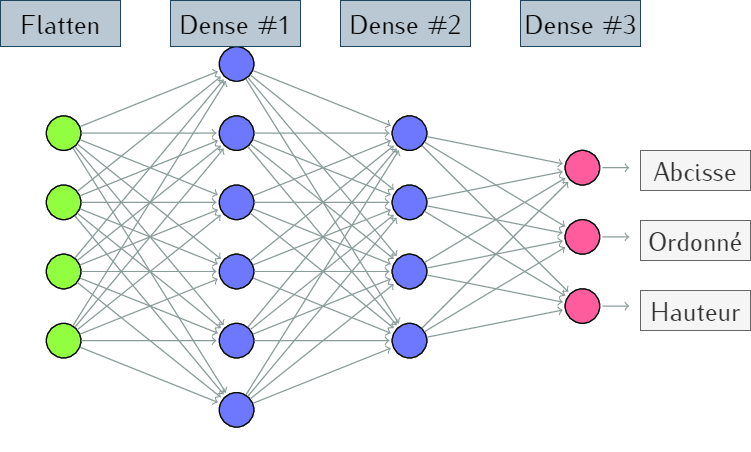
\includegraphics[width=.5\linewidth]{Dense} 
\decoRule
\caption[Dense]{Série de 3 couches denses « fully connected ». La couche en vert représente le résultat de l'opération de Flatten susmentionnée. L'utilisation des couches denses constitue la dernière étape des réseaux en figures \ref{fig:DRNN1} et \ref{fig:DRNN2} (Image adaptée de \parencite{Reference9})}
\label{fig:Dense}
\end{figure}

%----------------------------------------------------------------------------------------

\section{Configuration de l'entrainement}
Keras propose une multitude d'options et d'hyper-paramètres pour tuner le modèle et son entrainement. Ceux qui ont été utilisés sont indiqués dans les sections suivantes.


\subsection{Les métriques}

\subsubsection{Loss MSE}
Pendant la génération des données, on a pris soin de ne pas introduire de données aberrantes. La MSE (Mean Squared Error) qui est plus élevée que la MAE (Mean Absolute Error) sur les valeurs aberrantes est donc la plus adaptée. Si les $\hat{y}_i$ désignent les prédictions et $y_i$ les véritables cibles (ou valeurs observées ou labels), la MSE se définit par :
\begin{equation}
 \text{MSE} = \frac{1}{n} \sum_{i=1}^{n} \left( y_i - \hat{y}_i \right)^2
 \label{eqn:MSE}
\end{equation}

\subsubsection{Coefficient de détermination $R^2$}
\label{subsub:R2}
Le coefficient de détermination $R^2$ est très important en statistique. On peut l'obtenir par la formule :
\begin{align}
 R^2 = 1 - \frac{SS_{res}}{SS_{tot}}
 \label{eqn:R2}
\end{align}
Avec
\begin{align*}
 \quad SS_{res} =  \sum_{i=1}^{n} \left( y_i - \hat{y}_i \right)^2 \quad \text{et} \quad SS_{tot} =  \sum_{i=1}^{n} \left( y_i - \bar{y} \right)^2 
\end{align*}
Ou $ \bar{y} = \sum_{i=1}^{n} y_i $ représente la moyenne des valeurs observées.

On peut remarquer que :
\begin{itemize}
 \item Si le modèle prédit les valeurs attendues (observées), le score $R^2$ vaut 1. 
 \item SI le modèle prédit toujours la valeur moyenne $\bar{y}$, le score $R^2$ vaut 0.
 \item Si les prédictions sont pires que la moyenne, le score $R^2$ est négatif.
\end{itemize}

En général, si les prédiction et les valeurs observées sont très corrélées (sans être égales), on aura un score $R^2$ qui n'est pas caractéristique des résultats. En effet, pour des tâches de régression, il se définit comme étant le carré du coefficient de corrélation entre les valeurs prédites et les valeurs observées.

Dans la suite de ce rapport, le score $R^2$ sera présenté sous forme de pourcentage. 

\subsubsection{Un score personnalisé}
On définit à présent un score particulièrement adapté à nos données. On déclare qu'une prédiction est correcte si elle est suffisamment proche du label :
\begin{itemize}
 \item \textbf{au dixième près} pour la position (suivant $x$ ou $y$) car le domaine d'étude est $[0,1]$ en 1D et $[0,1] \times [0,1]$ en 2D
 \item \textbf{à l'unité près} pour la hauteur car les hauteurs observées sont comprises entre 1 et 10 (en 1D) et 0.1 et 10 (en 2D) 
\end{itemize}

Le score personnalisé est donc un score sévère (pourcentage des prédictions correctes) qui récompense les prédictions qui sont à la fois précisent en hauteurs et en position.


\subsection{Les hyper-paramètres}

\subsubsection{L'optimiseur}
L'optimisation est une méthode d'accélération de l'entrainement. À la place de l'algorithme classique de descente de gradient stochastique, nous utiliserons l'optimiseur Adam\footnote{Adaptative moment estimation} qui combine les propriétés de deux autres algorithmes d'entrainement (AdaGrad et RMSProp) pour offrir une performance de taille.

\subsubsection{Activation ReLU}
La fonction d'activation introduit une non-linéaire entre les couche. L'avantage majeur de l'activation ReLU\footnote{Rectified Linear Unit} (que nous utiliserons) par rapport aux autres fonctions d'activation c'est qu'elle n'active pas tous les neurones en même temps. D'un point de vue computationnel, elle est très efficace tout en produisant des résultats satisfaisants.

\subsubsection{Le taux d'apprentissage}
Il s'agit du paramètre le plus influant pour notre apprentissage. Il contrôle à quelle vitesse le modèle s'adapte au problème, en déterminant de quelle quantité les poids des neurones seront mis à jour \footnote{Les poids des neurones ayant été initialisés de façon aléatoire} après l'algorithme de « backpropagation ». S'il est très élevé, il peut rapidement conduire à solution non optimale. S'il est très faible, le modèle peut resté figé (il faudra alors un nombre élevé d'époques pour potentiellement le débloquer). En 1D, nous avons utilisé un taux d'apprentissage égale à \verb|1e-4| alors qu'en 2D, nous l'avons pris égale à \verb|1e-5|.

\subsubsection{Le « batch size »}
Il s'agit de la taille de chaque paquet de données \footnote{Nombre d'instances d'entrainement (« samples ») sélectionnés aléatoirement} passé au modèle durant une époque. Un « batch size » faible apporte du bruit au modèle, dû au fait qu'une portion aléatoire des données est utilisée pour mettre à jour les poids des neurones. Ceci assure une meilleure généralisation du modèle tout en limitant la quantité de données chargée dans la RAM à chaque époque.

% 
% \subsubsection{le coefficient de reglarisation L2}
% Le penalisation permet d;eviter le surapprentissage. Sous Keras, on peut soit penaliser les poids d'une couche (kernel optimizer), ou bien penaliser les resultats de la fonction d'activation de cette couche (activity optimizer). la deuxieme option a offert les meilleures resultats, c'est pourquoi l'avons appliquee a nos deux couches de neuronnes denses  de nos modeles avec un coefficient de 1e-5.
% 

\subsubsection{Early-stopping}
La technique d'Early-stopping sera notre moyen primaire de lutte contre le sur-apprentissage\footnote{Lorsque le modèle s'ajuste trop précisément au jeu de données utilisé pour l'entrainer.}. Pour l'implémenter de façon efficace sous Keras, il nous faut une variable appelée "\verb|patience|" . Il s'agit du nombre d'époques à attendre avant d'arrêter l'apprentissage de façon précoce. Nous arrêterons nos entrainements dès que le score $R^2$ (voir paragraphe \ref{subsub:R2}) sur le jeu de validation (val) n'aura pas augmenté pendant 10 époques. 

%----------------------------------------------------------------------------------------

\section{Résultats}

Nous résumons la section précédente en spécifiant les hyper-paramètres (et leurs définitions) utilisés pour entrainer le modèle sous Keras.

\begin{table}[h!]
\caption{Liste des paramètres majeurs utilisés pour l'entrainement. L'activation "relu" est utilisée sur les couches cachées et "linear" sur la couche de sortie. Les paramètres non indiqués dans ce tableau (« pool size », etc.) sont pris par défaut sous Keras.}
\label{tab:Parametres}
\centering
\begin{tabular}{l l l}
\toprule
\tabhead{Hyper-paramètre} & \tabhead{Définition} & \tabhead{Valeur 1D / 2D} \\
\midrule
\verb|learning_rate| & taux d'apprentissage & 1e-4 / 1e-5\\
\verb|batch_size| & taille d'un batch a chaque époque  & 32\\
\verb|optimizer| & algorithme d'optimisation & Adam\\
\verb|activation| & type de fonction d'activation  & "relu" ou "linear"\\
\verb|patience| & patience pour l'\verb|early_stopping| & 10\\
\verb|epochs| & nombre d'époques & 100\\
\verb|kernel_size| & taille du noyau de convolution & 3 / (6,2)\\
\bottomrule\\
\end{tabular}
\end{table}


Nous avons entrainé les architectures en 1D et 2D en ajustant convenablement les dimensions des couches d'entrée et de sortie. Observons à présent les résultats obtenus sur le jeu de données test.

\subsection{Régression}
% 
    \subsubsection{En 1D}
    On obtient de très bonnes prédictions sur la hauteur de l'obstacle car celle-ci affecte directement l'amplitude des signaux sur le bord droit du domaine. Cela se traduit par un score $R^2$ très élevé. Mais ce score n'est pas assez indicatif vu que les prédictions sur la position du créneau de densité ne sont pas bonnes \footnote{Le score $R^2$ élevé pourrait s'expliquer par le fait que le poids de la hauteur dans la corrélation est plus fort que celui de la position.}. Le score personnalisé permet de capturer ce défaut et donne environ 25 \% (voir \ref{tab:Tab1D}).
    
    \begin{table}[h!]
    \caption{Résultats obtenus sur le jeu test en 1D. Le modèle avec Max-poling correspond à la figure \ref{fig:DRNN1}, et celui sans Max-pooling à la figure \ref{fig:DRNN2}, tous deux implémentés pour des données 1D. Ces valeurs représentent une moyenne obtenue sur plusieurs cycles d'entrainement/prédiction.}
    \label{tab:Tab1D}
    \centering
    \begin{tabular}{l l l}
    \toprule
    \tabhead{Score} & \tabhead{Avec Max-pooling} & \tabhead{Sans Max-pooling} \\
    \midrule
    $R^2$ & 99.49 \% & 99.50 \%\\
    Personnalisé & 26.50 \% & 28.21 \%\\
    \bottomrule\\
    \end{tabular}
    \end{table}

    \begin{figure}[!h]
    \begin{subfigure}{.5\textwidth}
    \centering
    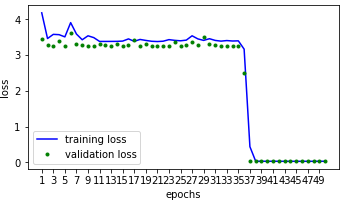
\includegraphics[width=.8\linewidth]{1DPool}  
    \caption[2DPool]{Avec Max-pooling}
    \end{subfigure}
    \begin{subfigure}{.5\textwidth}
    \centering
    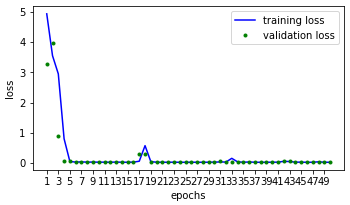
\includegraphics[width=.8\linewidth]{1DNoPool}  
    \caption[2DNoPool]{Sans Max-pooling}
    \end{subfigure}
    \label{fig:1DLoss}

    \centering
    \decoRule
    \caption[Loss 1D]{Comparaison de la vitesse de décroissance de la loss en 1D}
    \end{figure}

    Même si aucun n'est capable de correctement prédire la position du créneau, le modèle sans Max-pooling semble mieux se comporter sur notre jeu de données. Pour les illustrations qui vont suivre, nous utiliserons donc ce dernier modèle (sans Max-pooling). Nous commençons par une illustration de la corrélation entre les labels et les prédictions (figure \ref{fig:Illustration1D}).
    
    \begin{figure}[!h]
    \begin{subfigure}{.5\textwidth}
    \centering
    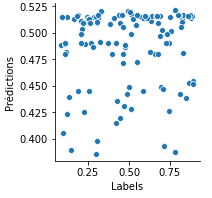
\includegraphics[width=.5\linewidth]{Position1D}  
    \caption[Pos1D]{Position}
    \end{subfigure}
    \begin{subfigure}{.5\textwidth}
    \centering
    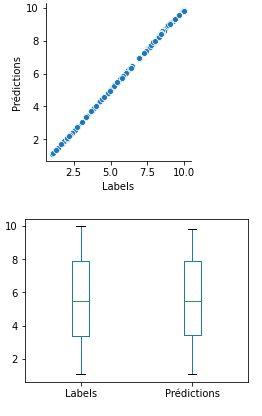
\includegraphics[width=.5\linewidth]{Hauteur1D}  
    \caption[H1D]{Hauteur}
    \end{subfigure}
    
     \centering
    \decoRule
    \caption[Illustration 1D]{Illustration de la corrélation entre les labels et les prédictions obtenues par le modèle sans Max-pooling en 1D. On peut observer l'exactitude des prédictions pour la hauteur (B) mais un échec sur la position (A). En effet, les prédictions de la position du créneau sont concentrée autour de la moyenne 0.5.}
    \label{fig:Illustration1D}
    \end{figure}

    Pour observer les meilleures et les pires prédictions du modèle, il nous faut une mesure de la distance entre les prédiction et les labels. On définit donc la norme ci-bas (en prenant soins de normaliser la hauteur). $$ \text{Norme} = \sqrt{\text{Position}^2 + \left( \frac{\text{Hauteur}}{10} \right)^2}$$
    
    Observons donc les meilleures prédictions du modèle (sans Max-pooling) (figure \ref{fig:Meilleur1D}).
    \begin{figure}[!h]
    \begin{subfigure}{.5\textwidth}
    \centering
    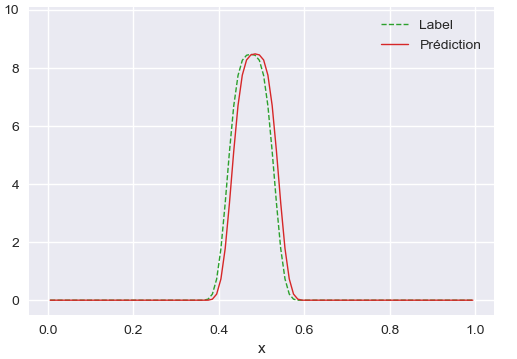
\includegraphics[width=.8\linewidth]{Meilleur1D1}  
    \caption[Meilleur1D1]{Label = [0.488 8.474] \\ Prédiction = [0.49  8.486]}
    \end{subfigure}
    \begin{subfigure}{.5\textwidth}
    \centering
    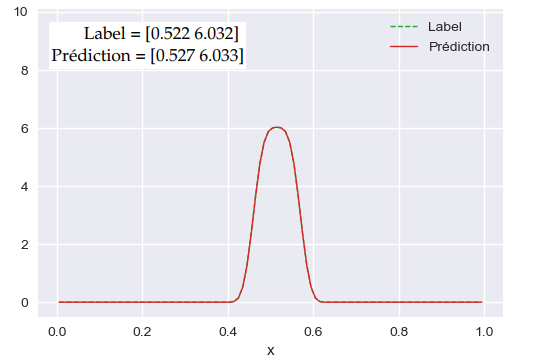
\includegraphics[width=.8\linewidth]{Meilleur1D2}  
    \caption[Meilleur1D2]{Label = [0.522 6.032]  \\ Prédiction = [0.527 6.033]}
    \end{subfigure}
    
     \centering
    \decoRule
    \caption[Meilleur 1D]{Les meilleures prédictions 1D. Il s'agit ici d'une reconstruction manuelle de la densité du milieu à partir des vecteurs en titre des figures (A) et (B). La première coordonnée indique la position du saut de densité, et la deuxième sa hauteur. On confirme que les bonnes prédictions des positions sont proches du milieu du domaine.}
    \label{fig:Meilleur1D}
    \end{figure}
    
    Les pires prédictions du modèle permettent de mieux illustrer les problèmes rencontrés avec l'apprentissage 1D (figure \ref{fig:Pire1D}).
    
    \begin{figure}[H]
    \begin{subfigure}{.5\textwidth}
    \centering
    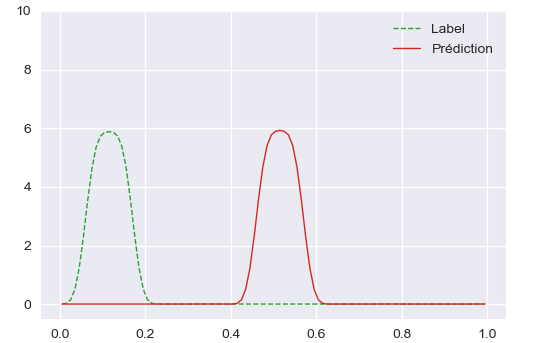
\includegraphics[width=.8\linewidth]{Pire1D1}  
    \caption[Pire1D1]{Label = [0.125 5.886] \\ Prédiction = [0.524 5.925]}
    \end{subfigure}
    \begin{subfigure}{.5\textwidth}
    \centering
    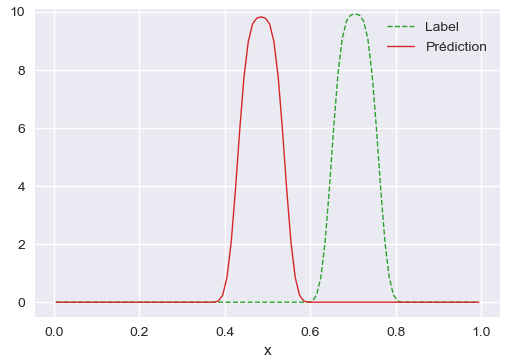
\includegraphics[width=.8\linewidth]{Pire1D2}  
    \caption[Pire1D2]{Label = [0.892 8.195]  \\ Prédiction = [0.454 8.167]}
    \end{subfigure}

     \centering
    \decoRule
    \caption[Pire1D]{Les pires prédictions du modèle 1D (sans Max-pooling). La différence se joue au niveau de la position du créneau comme indiquée à la figure \ref{fig:Illustration1D}. Les labels les plus éloignés du milieu conduisent aux prédictions les plus mauvaises.}
    \label{fig:Pire1D}
    \end{figure}
%     - 3eme pire prediction: label [0.302 1.066]     prediction [0.503 1.144]
    
    La faible précision obtenue est due au fait que la simulation 1D est quasiment invariante par translation. En effet, une variation de la position du créneau de densité ne change les signaux sur la droite que de très peu. Ceci est probablement dû au fait que le problème inverse est mal posé, dans le sens ou il n'y a pas unicité de la solution. Pour améliorer le score personnalisé, on pourrait passer en 2D.
    
    \subsubsection{En 2D}
    En 1D, on ne mesurerait la sortie que sur 1 seul bord du domaine, ce qui limitait beaucoup l'apprentissage. En 2D, on récupère beaucoup plus d'informations (4 bords, 4 positions distinctes de la source) et cela renforce les chances d'unicité de la solution du problème inverse. 

    Comme attendu, le réseau est capable de détecter non seulement la hauteur de l'obstacle, mais aussi son abscisse et son ordonnée. Notre score personnalisé nous permet de confirmer cela dans le tableau \ref{tab:Tab2D}.
    
    \begin{table}[h!]
    \caption{Résultats obtenus sur le jeu test en 2D}
    \label{tab:Tab2D}
    \centering
    \begin{tabular}{l l l}
    \toprule
    \tabhead{Score} & \tabhead{Avec Max-pooling} & \tabhead{Sans Max-pooling} \\
    \midrule
    $R^2$ & 94.80 \% & 98.81 \%\\
    Personnalisé & 55.75 \% & 93.50 \%\\
    \bottomrule\\
    \end{tabular}
    \end{table}

    On constate que le modèles sans l'opération de Max-pooling est globalement meilleur que son homologue avec Max-pooling, dû à l'application de l'Early-stopping. La figure \ref{fig:2DLoss} permet d'observer cela à travers la vitesse de convergence du modèle.
    
    \begin{figure}[!h]
    \begin{subfigure}{.5\textwidth}
    \centering
    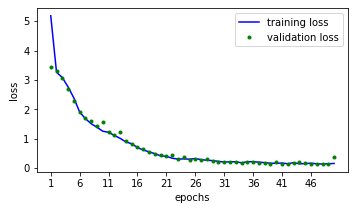
\includegraphics[width=.8\linewidth]{2DLossPool}  
    \caption[2DPool]{2D avec Max-pooling}
    \end{subfigure}
    \begin{subfigure}{.5\textwidth}
    \centering
    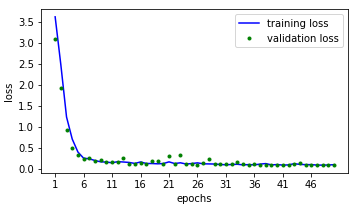
\includegraphics[width=.8\linewidth]{2DLossNoPool}  
    \caption[2DNoPool]{2D sans Max-pooling}
    \end{subfigure}

    \centering
    \decoRule
    \caption[Loss en 2D]{Comparaison de la vitesse de décroissance de la loss en 2D}
    \label{fig:2DLoss}
    \end{figure}

    Comme nous l'avons fait en 1D, Le modèle sans Max-pooling sera utilisé par la suite pour illustrer la corrélation entre les prédictions (de l'abscisse $x$, de l'ordonne $y$, et de la hauteur) et leurs labels respectifs (figure \ref{fig:Illustration2D}).
    \begin{figure}[!h]
    \begin{subfigure}{.33\textwidth}
    \centering
    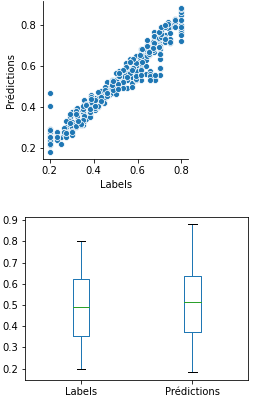
\includegraphics[width=.7\linewidth]{PositionX2D}  
    \caption[PosX2D]{Abscisse}
    \end{subfigure}
    \begin{subfigure}{.33\textwidth}
    \centering
    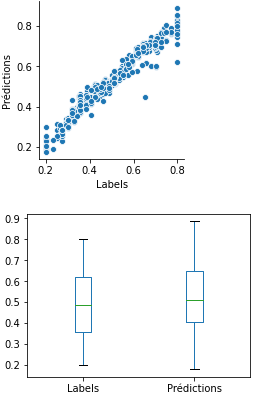
\includegraphics[width=.7\linewidth]{PositionY2D}  
    \caption[PosY2D]{Ordonnée}
    \end{subfigure}
    \begin{subfigure}{.33\textwidth}
    \centering
    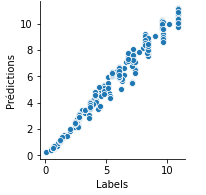
\includegraphics[width=.7\linewidth]{Hauteur2D}  
    \caption[H2D]{Hauteur}
    \end{subfigure}
    
     \centering
    \decoRule
    \caption[Illustration 2D]{Illustration de la corrélation entre les labels et les prédictions obtenues par le modèle sans Max-pooling en 2D. On peut observer que toutes les trois informations sont relativement bien corrélées, d'où le score $R^2$ élevé (voir tableau \ref{tab:Tab2D}).}
    \label{fig:Illustration2D}
    \end{figure}
    
    Pour observer les meilleures et les pires prédictions du modèle, on définit donc la norme ci-bas. $$ \text{Norme} = \sqrt{\text{Abcisse}^2 + \text{Ordonee}^2 + \left( \frac{\text{Hauteur}}{10} \right)^2}$$
    
    \begin{figure}[!h]
    \begin{subfigure}{.5\textwidth}
    \centering
    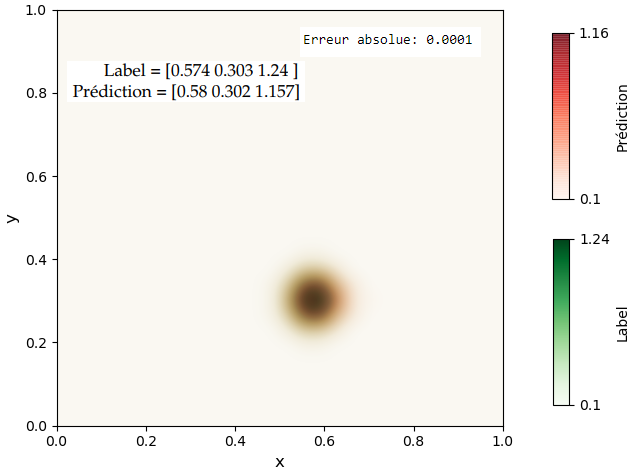
\includegraphics[width=.8\linewidth]{Meilleur2D1}  
    \caption[Meilleur2D1]{Label = [0.574 0.303 1.24 ] \\ Prédiction = [0.58  0.302 1.157]}
    \end{subfigure}
    \begin{subfigure}{.5\textwidth}
    \centering
    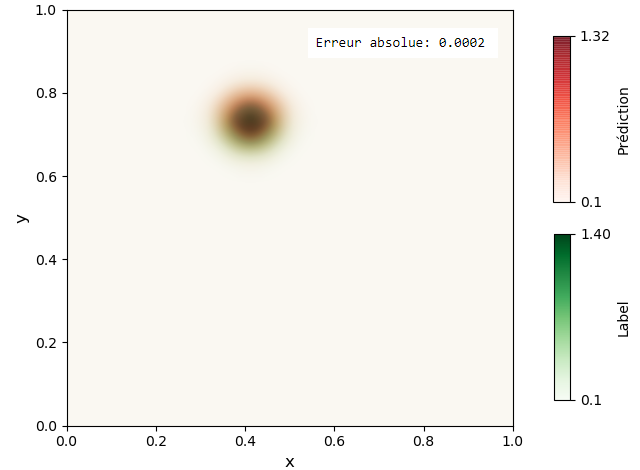
\includegraphics[width=.8\linewidth]{Meilleur2D2}  
    \caption[Meilleur2D2]{Label = [0.405 0.724 1.392]  \\  Prédiction = [0.409 0.736 1.318]}
    \end{subfigure}
    
     \centering
    \decoRule
    \caption[Meilleur 2D]{Les meilleures prédictions 2D. Ces images ont été reconstruites à partir des vecteurs "Labels" et "Prédiction" issus de l'apprentissage. La première coordonnée indique l'abscisse $x$ du saut de densité, la deuxième son ordonnée $y$, et la troisième sa hauteur. L'interpolation bicubique a été utilisée pour obtenir des images plus nettes.}
    \label{fig:Meilleur2D}
    \end{figure}

    \begin{figure}[H]
    \begin{subfigure}{.33\textwidth}
    \centering
    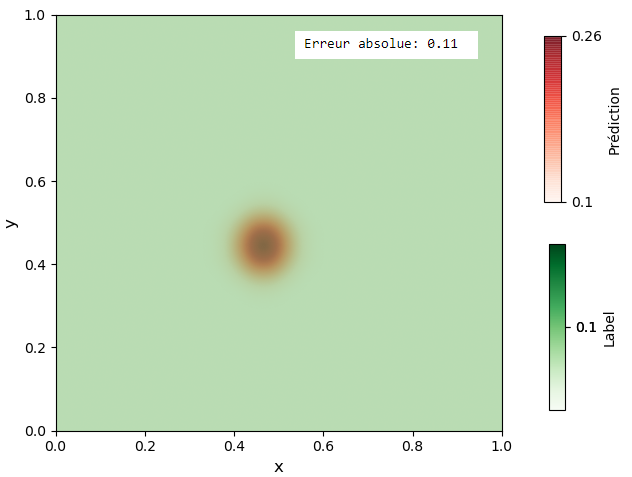
\includegraphics[width=1\linewidth]{Pire2D1}  
    \caption[Pire2D1]{Label = [0.2  0.65 0.1 ] \\ Prédiction = [0.466 0.448 0.267]}
    \end{subfigure}
    \begin{subfigure}{.33\textwidth}
    \centering
    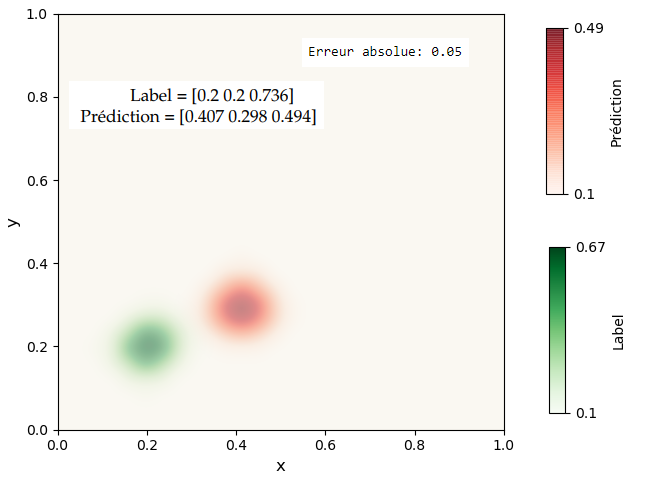
\includegraphics[width=1\linewidth]{Pire2D2}  
    \caption[Pire2D2]{Label = [0.2   0.2   0.736]  \\ Prédiction = [0.407 0.298 0.494]}
    \end{subfigure}
    \begin{subfigure}{.33\textwidth}
    \centering
    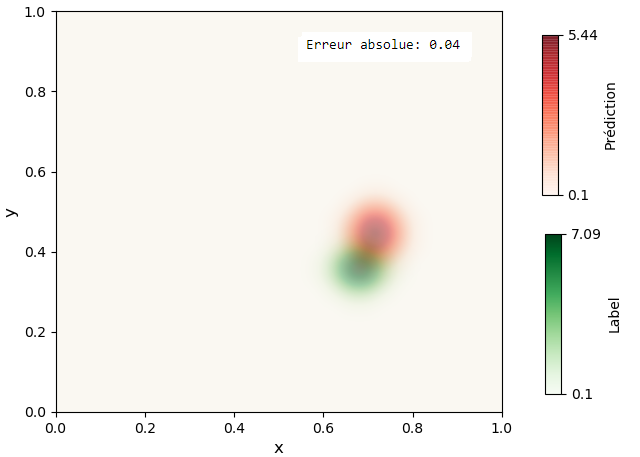
\includegraphics[width=1\linewidth]{Pire2D3}  
    \caption[Pire2D3]{Label = [0.674 0.358 7.096]  \\ Prédication = [0.712 0.449 5.462]}
    \end{subfigure}

     \centering
    \decoRule
    \caption[Pire2D]{Les pires prédictions du modèle 2D. Sans surprise la plus mauvaise des prédictions s'obtient lorsque le créneau est absent (A). En général, les pires prédictions sont faites lorsque le créneau se situe très proche de l'extrémité du domaine(B). La figure (C) représente un cas particulièrement mauvais de prédiction de la hauteur du créneau.}
    \label{fig:Pire2D}
    \end{figure}
    
    En ce qui concerne la généralisation du modèle à d'autres formes d'obstacles, je n'ai pas eu l'occasion de comparer les modèles avec et sans Max-pooling. Le modèle sans Max-pooling risque alors d'être moins performant conformément à la théorie (voir paragraphe \ref{subsec:MaxPoling}). Sous Keras, le modèle à prouver être capable d'apprendre en continu, du moment que les entrées sont toutes normalisées et ont la même forme.

\subsection{Classification}
\label{sec:Classif}
Une deuxième piste étudiée durant le stage a été la classification mutilabel sur les données 2D. L'idée est de déterminer l'ordonnée de l'obstacle en trouvant en face de quelle(s) source(s) il est placé. La structure des entrées est quasiment la même que pour la régression en 2D (voir figure \ref{fig:entreesortie2D}), sauf qu'il manque les signaux sur la gauche (coté où se trouve la source). En ce qui concerne les sorties, l'image ci-dessous décrit mieux leur structure :

\begin{figure}[!h] 
\centering
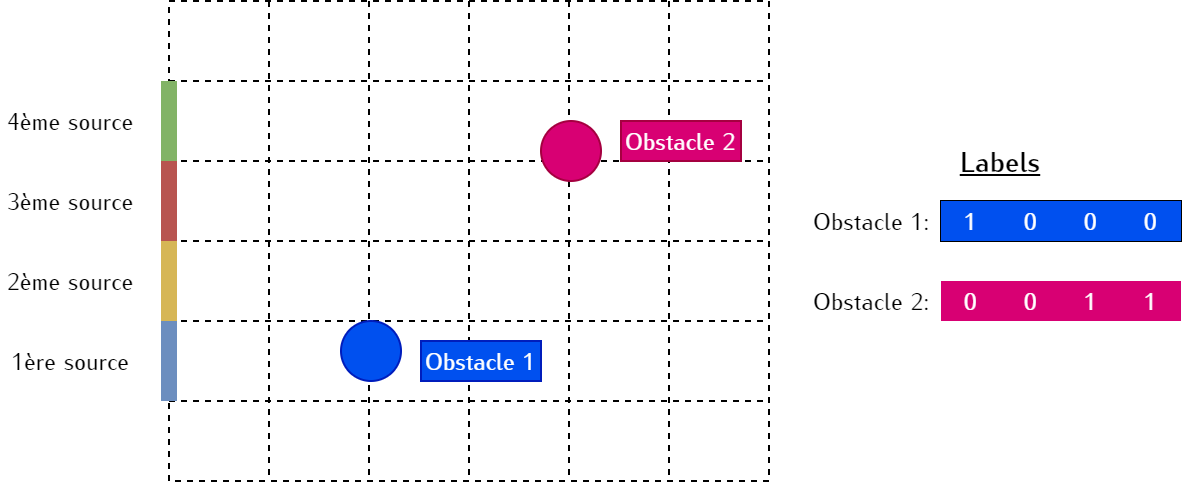
\includegraphics[width=.8\linewidth]{Classification} 
\decoRule
\caption[Classification]{Description des labels pour la classification multilabel en 2D. Un label est marque 1 si l'obstacle se trouve dans le champ de la source correspondante, et 0 sinon.}
\label{fig:Classification}
\end{figure}

Bien qu'ils aient une structure similaire, la taille des données utilisées pour la classification est différente de celle des données utilisées pour la régression (voir figure \ref{fig:entrees2D}). On a moins d'itérations en temps (40 au lieu de 168) mais un maillage beaucoup plus fin (90x90 au lieu de 28x28). Le modèle de CNN utilisé ressemble beaucoup à celui utilisé pour la régression 2D. Une importante différence est qu'on utilise une activation "sigmoid" à la place de l'activation "linear" au niveau de la couche de sortie. On obtient donc en sortie des probabilités qu'il faut séparer en 2 classes suivant un seuil. Le modèle est entrainé avec des hyper-paramètres identiques à ceux utilisés durant la régression 2D. Les résultats sont présentés dans la table \ref{tab:Class}.

\begin{table}[h!]
\caption{Résultats obtenus pour la classification en 2D. Le score sévère favorise les prédictions qui sont égales au véritable label sur toutes les 4 colonnes. Un seuillage convenablement effectué permet d'augmenter la précision des résultats. Le score de « Binary accuracy » procuré par Keras est calculé avant le seuillage.}
\label{tab:Class}
\centering
\begin{tabular}{l l l}
\toprule
\tabhead{Score} & \tabhead{Avec Max-pooling} & \tabhead{Sans Max-pooling} \\
\midrule
Binary accuracy & 75.00 \% & 98.86 \%\\
Score sévère après seuillage & 27.27 \% & 95.45 \%\\
\bottomrule\\
\end{tabular}
\end{table}

\begin{figure}[!h]
\begin{subfigure}{.5\textwidth}
\centering
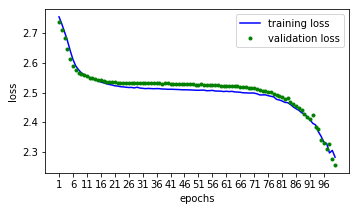
\includegraphics[width=.8\linewidth]{ClassPool}  
\caption[2DPool]{2D avec Max-pooling}
\end{subfigure}
\begin{subfigure}{.5\textwidth}
\centering
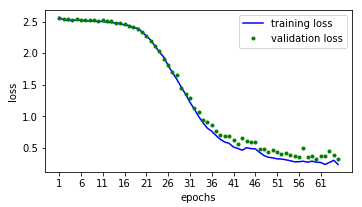
\includegraphics[width=.8\linewidth]{ClassNoPool}  
\caption[2DNoPool]{2D sans Max-pooling}
\end{subfigure}

\centering
\decoRule
\caption[ClassLoss]{Comparaison de la vitesse de décroissance de la loss (Multilabel Crossentropy) pour la classification en 2D}
\label{fig:ClassLoss}
\end{figure}


\begin{figure}[H] 
\centering
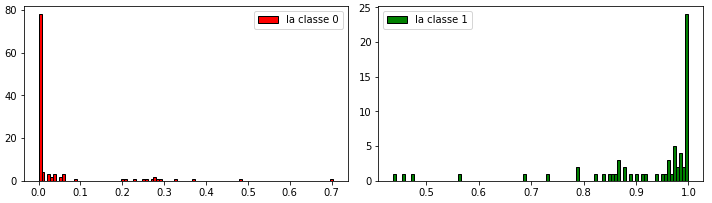
\includegraphics[width=.8\linewidth]{ClassFiabilite} 
\decoRule
\caption[ClassFiabilite]{Confiance du modèle sans Max-pooling en ses prédication. En rouge la classe 0 qui indique l'absence du créneau devant la source, et en vert la classe 1. Cette figure indique que le modèle se trompe très rarement, ce qui confirme le résultat obtenu au tableau \ref{tab:Class}.}
\label{fig:ClassFiabilite}
\end{figure}


Dans ce cas aussi, le modèle sans Max-pooling semble meilleur (figures \ref{fig:ClassLoss} et \ref{fig:ClassFiabilite}). Cependant nous ne disposons pas d'assez de données pour vérifier celui qui se généralise le mieux. Ceci étant une classification, les meilleures prédictions du modèle sont exactement les labels attendus et les pires prédictions ne diffèrent que de peu (de 1) de leurs cibles. Il est intéressant de constater qu'il n'y a aucune prédiction aberrante, par exemple : un obstacle se trouve en face des sources 1 et 3 sans recontrer la source 2.

La classification est très prometteuse. Cependant elle n'offre pas beaucoup de précision car nous n'avons utilisé que quatre sources. Ceci constitue une grande limitation pour cette méthode, surtout dans des cas pratiques. En milieu médical par exemple, la localisation d'une tumeur se veut très précise. Pour remédier à ce problème, on pourrait augmenter le nombre de sources sur la gauche et en placer d'autres suivant la verticale. Il faudra penser à sous-échantillonner davantage les entrées car l'augmentation des sources est très coûteuse en espace mémoire (pour les données et pour les poids du modèle de CNN). 

%----------------------------------------------------------------------------------------

\section{Conclusion sur l'apprentissage}
Nous avons essentiellement effectué trois apprentissages durant le stage. Par ordre croissant de réussite, nous avons :

\begin{enumerate}
  \item \textbf{Régression 1D} : Elle a permis de détecter la hauteur du créneau sur la densité d'un domaine 1D (avec la meilleure corrélation de tous les apprentissages). Elle n'a cependant pas été capable de détecter la position du créneau, probablement dû au caractère mal posé du problème inverse.
  \item \textbf{Classification 2D} : Elle a permis de localiser l'ordonnée du créneau en le situant par rapport aux sources sur la gauche d'un domaine 2D. En augmentant leur nombre et en plaçant certaines sources en haut (ou en bas) du domaine, on pourrait localiser avec plus de finesse l'abscisse et l'ordonnée du créneau.
  \item \textbf{Régression 2D} : Elle a permis de prédire tous les attributs essentiels du créneau (abscisse, ordonnée, et hauteur), tout ceci avec une très forte précision (score personnalisé s'élevant à 93 \%). 
\end{enumerate}

Durant chacun de ces apprentissages, nous avons comparé des modèles avec et sans Max-pooling en vue d'étudier la généralisation à d'autres formes d'obstacles et d'opacités. Le modèle sans Max-pooling a prouvé être supérieur dans le cas que nous avions à notre disposition.